\chapter{Plan de trabajo}
Mi trabajo se ha centrado en mejorar la herramienta en los aspectos gráficos y funcionales, y añadiendo en la medida de lo posible todas las funcionalidades que hemos considerado necesarias para la aplicación.

A continuación se describen con detalles los principales cambios y mejoras que se han implementado con respecto a la versión anterior.
%%%%%%%%%%%%%%%%
\section{Cambios a nivel de diseño}
\begin{figure}[H]
    \centering
    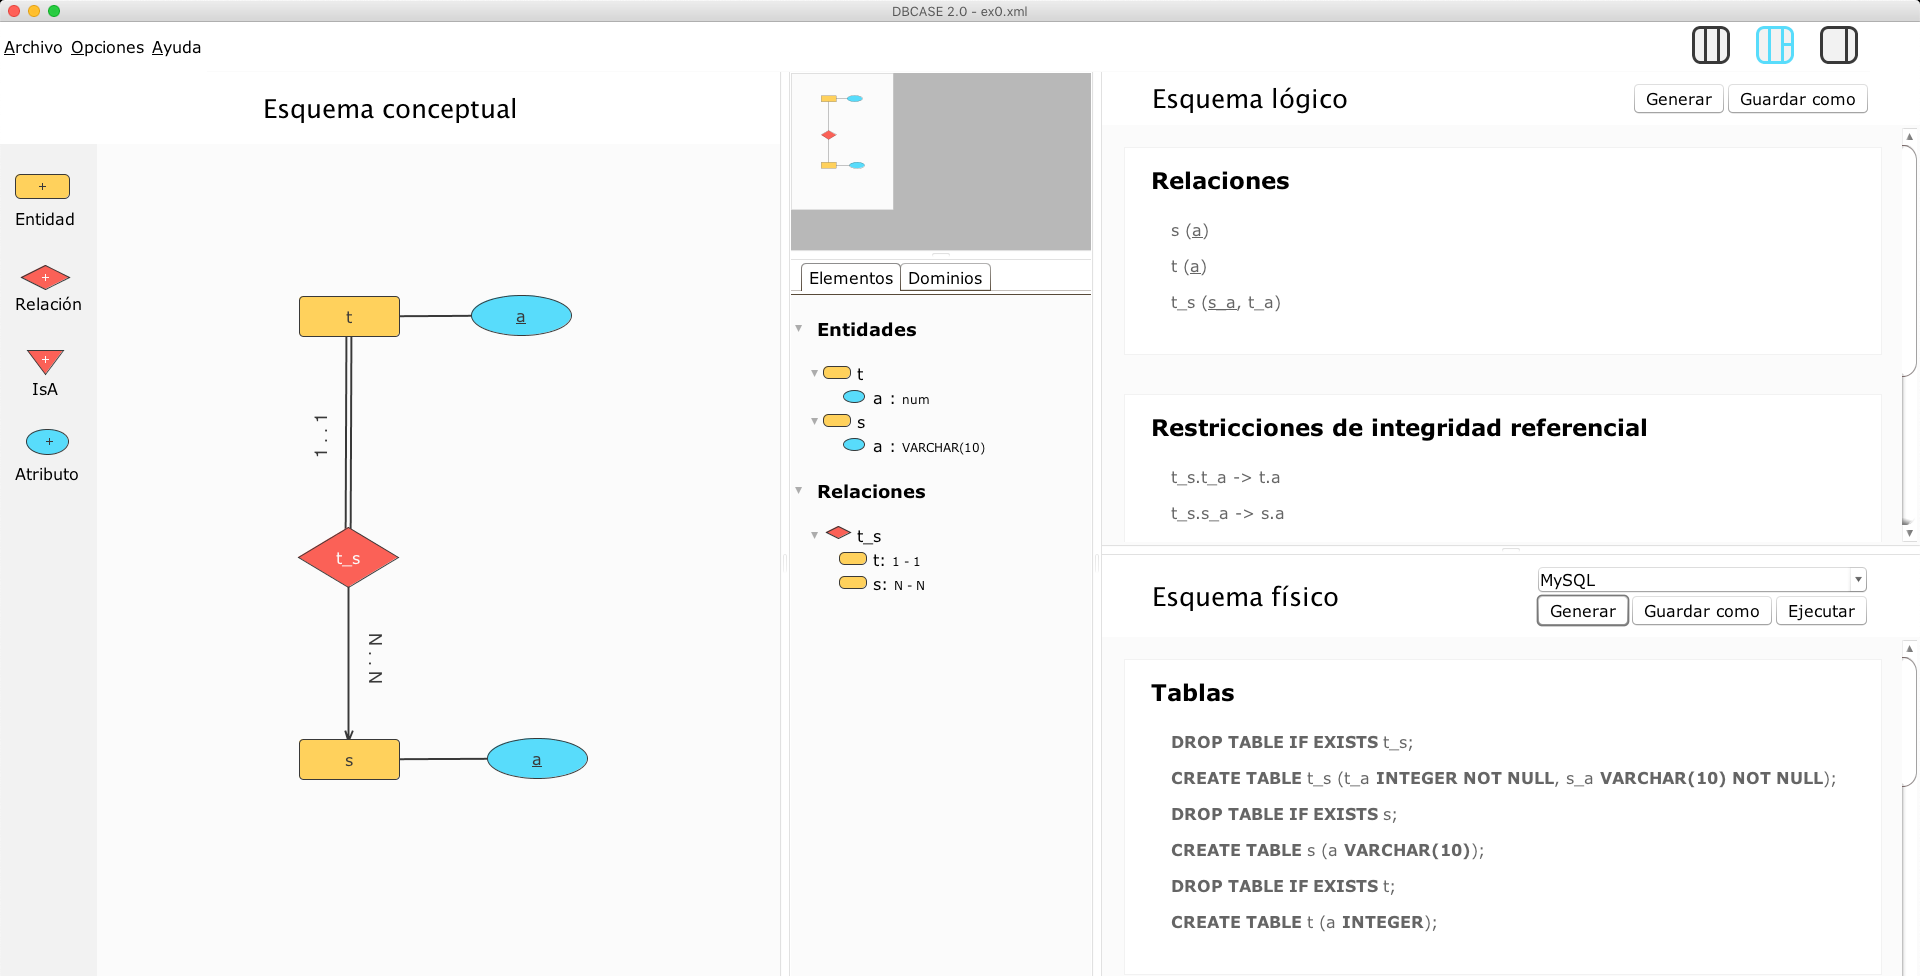
\includegraphics[width=\textwidth]{img/GUI_DBCASE.png}
    \caption{GUI de DBCASE 2.0}
\end{figure}
La aplicación ha sufrido un profundo cambio de diseño. Se ha buscado dar un aspecto más moderno a la aplicación, de forma que se han conservado las librerías gráficas con las que implementó y se ha intentado exprimir al máximo sus posibilidades.\\

\subsection{Look and Feel}
Debido a la decisión de continuar usando las librerías de java swing, se investigaron las posibilidades que ofrecía para personalizar el diseño de la interfaz. Una de las principales opciones que ofrece java swing es la de poder editar fácilmente el estilo de los paneles mediante el denominado look and feel.

\begin{lstlisting}[backgroundcolor = \color{white},
                   xleftmargin = 2cm,language=java,basicstyle=\medium]
javax.swing.UIManager.setLookAndFeel();
\end{lstlisting}

El look and feel en java swing permite cambiar el aspecto por defecto de todos los componentes visuales generados por la librería (JPanel, JFileChooser, JFrame, etc).

\subsubsection{Nimbus Look and Feel}
Java ofrece por defecto varios look and feel con los que el programador puede editar sus interfaces.\\

De las distintas opciones se decidió utilizar Nimbus Look and Feel.
\begin{quote}
    \textit{"Nimbus es un pulido Look and Feel multiplataforma introducido en Java SE 6 Update 10 (6u10)."}\cite{nimbus}
\end{quote}

Entre los principales motivos que llevaron a tomar esta decisión destacan:
\begin{itemize}
    \item Su aspecto moderno y redondeado suponía un importante lavado de cara con respecto al aspecto anterior, y era una cualidad diferencial con respecto a las otras opciones.
    \item El hecho de que sea multiplataforma permite que la aplicación tenga un aspecto uniforme en los distintos sistemas operativos.
    \item La capacidad de personalización, que permite elegir el aspecto de prácticamente cualquier elemento visual de la interfaz.
\end{itemize}
\subsubsection{Nimbus Look and Feel personalizado}
La personalización de Nimbus se ha centrado principalmente en dos aspectos.
\begin{itemize}
    \item La fuente de texto: se ha buscado que la aplicación sea lo más accesible y clara posible, por lo que se ha utilizado la fuente \textbf{Verdana 16}, por ser una de las más usadas y simples, y a tamaño 16 para que la lectura por parte del usuario se realice sin dificultades.
    \item Los colores de los elementos, paneles, botones y menús. De forma que permitiera la implementación de distintos temas.
\end{itemize}

\subsection{Temas}
Un aspecto en el que se ha centrado el trabajo ha sido en la implementación de temas que permitieran al usuario personalizar la interfaz gráfica.\\

Los dos objetivos que se perseguían con la implementación de temas eran:
\begin{itemize}
    \item Habilitar un tema oscuro, tan usado en las interfaces de usuario modernas, que permite reducir la fatiga visual y hace más cómodo el trabajo en entornos con poca luz.
    \item Permitir a los usuarios crear y personalizar sus propios temas, pudiendo escoger los colores principales que utiliza la aplicación.
\end{itemize}
\subsubsection{Detalles de la implementación de los temas}
Para que la creación y personalización de temas fuera lo más dinámica posible se decidió que los distintos temas se almacenasen en archivos \textbf{json}\cite{json}, externos al programa, de forma que el usuario pueda modificarlos, copiarlos o eliminarlos fácilmente. Los archivos json que contienen los temas se almacenan en la carpeta "themes".\\

\begin{quote}
\textit{"JSON (acrónimo de JavaScript Object Notation) es un formato de texto sencillo para el intercambio de datos."}
\end{quote}

Dentro del archivo json, se establecen el nombre del tema, y los colores de los principales elementos de la aplicación, entre ellos algunos de los más destacables son:
\begin{itemize}
    \item El color de los elementos del diagrama (relaciones, atributos y entidades).
    \item El color de fondo del diagrama.
    \item El color principal de la aplicación (utilizado por Nimbus para pintar el fondo de los paneles, botones, etc).
    \item El color de las fuentes, tanto de la fuente de los paneles como de la fuente de los cuadros de texto de los esquemas relacional y físico.
\end{itemize}

Dentro del menú de opciones, el usuario tiene la posibilidad de elegir un tema de entre todos los temas disponibles dentro de la carpeta "themes".\\

Se han incorporado dos temas con la aplicación:
\begin{itemize}
    \item \textbf{Light} o tema claro: es el tema por defecto. Utiliza colores blancos y grises para la aplicación, y colores elementales para resaltar los elementos del diagrama.
    \item \textbf{Dark} o tema oscuro: tiñe la interfaz con colores negros manteniendo el protagonismo de los elementos del diagrama.
\end{itemize}

Además el usuario puede crear sus propios temas añadiendo un archivo en formato json a la carpeta "themes" que siga la estructura de los temas incorporados.\\

Para el manejo interno de los temas se ha creado una clase theme utilizando el patrón de diseño \textbf{"Singleton"}\cite{singleton}, lo que permite a cualquier otra clase obtener una instancia de la misma y poder consultar en ella los colores de forma sencilla.

\subsection{Disposición de paneles}
Uno de los mayores cambios que ha sufrido la interfaz de usuario ha sido la disposición de los distintos paneles. Se ha buscado una GUI más clara y sencilla sin perder ninguna de las funcionalidades.\\

Con respecto a la versión anterior, los cambios principales que ha sufrido la interfaz son:
\begin{itemize}
    \item Se ha pasado de una interfaz dividida en dos pestañas (diagrama entidad-relación y generación de código) a una sola, de forma que ahora se puede ver de un vistazo el diagrama y el código generado.
    \item El panel de generación de código se ha dividido en dos paneles distintos: Esquema lógico y esquema físico. De esta manera quedan ambos lenguajes en paneles independientes.
    \item Se han unificado el panel de información y el panel de dominios en un solo JTabbedPane.
\end{itemize}
\subsection{Panel de información}

\begin{figure}[H]
    \centering
    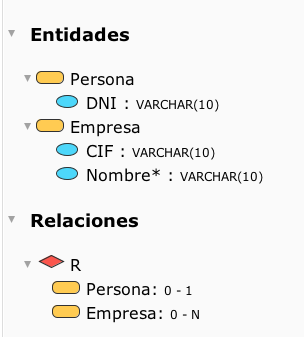
\includegraphics[width=0.4\textwidth]{img/PanelInfo.png}
    \caption{Panel de Información}
\end{figure}

El panel de información muestra un esquema en forma de arbol del modelo entidad relación existente en el panel de diseño, y en él se puede ver de forma esquemática todos los elementos y cómo están relacionados.\\

El panel de información ha sufrido profundos cambios que se describen a continuación:

\begin{itemize}
    \item Ahora el panel muestra en todo momento la información global de todo el esquema creado por el usuario, al contrario que en la versión anterior, en la que solo mostraba la información de los elementos seleccionados.
    \item El panel de información ha pasado a dividirse en dos sectores: entidades y relaciones.
    \begin{itemize}
        \item \textbf{Entidades}: muestra todas las entidades del esquema y sus atributos. Muestra el dominio del atributo al lado del nombre y representa gráficamente de forma correcta los subatributos de atributos compuestos (como ramas de los mismos).
        \item \textbf{Relaciones}: muestra todas las relaciones del esquema y para cada una de ellas muestra sus atributos y las entidades que relaciona. Para cada una de las entidades muestra la cardinalidad al lado del nombre.\\
        
        Para las relaciones ISA muestra la entidad padre como la primera entidad de la relación, y las entidades hijas con un icono que las diferencia como tal.
    \end{itemize}
    \item Para la renderización del árbol (implementado con la clase JTree), se ha creado una clase personalizada que hereda de la clase DefaultTreeCellRenderer. Con ella se ha podido personalizar los iconos y las fuentes de cada uno de los elementos del árbol en función de su tipo. Los distintos iconos son generados mediante la clase Graphics2D \cite{g2d}, de forma que se evita el uso de imágenes externas pregeneradas, y permite que los colores de los iconos se adapten al tema seleccionado.
\end{itemize}

\subsection{Panel de dominios}
El panel de dominios informa al usuario de las opciones disponibles que tiene el usuario para asociar con los atributos creados. En este panel se han realizado los siguientes cambios.
\begin{itemize}
    \item El panel tiene un mayor tamaño y ahora muestra todos los dominios disponibles en el sistema, no solo los creados por el usuario.
    \item Solo para los dominios creados manualmente se muestra el conjunto de elementos disponibles y el tipo base al que pertenece el dominio, manteniendo la capacidad de editarlos.
    \item Se ha creado un nuevo renderizador para representar gráficamente el árbol, eliminando los iconos de ficheros de la versión anterior y dejando una interfaz más limpia e intuitiva.
    \item Se ha habilitado un botón para añadir nuevos dominios al sistema de forma sencilla.
\end{itemize}

\subsection{Barra lateral para añadir elementos}
\begin{figure}[H]
    \centering
    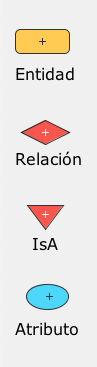
\includegraphics[width=0.15\textwidth]{img/barra_lateral.png}
    \caption{Barra lateral para añadir elementos}
\end{figure}
Dentro del área de diseño se ha añadido una barra lateral que permite agregar nuevos elementos al diagrama. De esta forma se consigue que el usuario pueda crear elementos nuevos de una forma más intuitiva que haciendo clic derecho sobre el panel de diagrama. A continuación se detallan las principales características de este panel.

\begin{itemize}
    \item Permite al usuario añadir cuatro tipos de elementos: entidades, relaciones, relaciones ISA y atributos.\\
    
    Los botones de añadir entidad y añadir relación muestran el cuadro de diálogo correspondiente, en el que se permite insertar el nombre y las características del elemento.\\
    
    El botón ISA, al no necesitar nombre ni configuración, inserta directamente la relación en el diagrama.\\
    
    El botón atributo permite seleccionar mediante un menú desplegable a qué entidad o relación pertenece el atributo, también se le pide al usuario el nombre y las características del atributo.
    \item Los elementos se insertan automáticamente en el diagrama. Al no haber hecho clic derecho el usuario en ningún punto del diagrama, el programa no dispone de una posición de referencia en la que el elemento debe ser insertado. Por ello el programa genera unas coordenadas automáticamente.
    \begin{itemize}
        \item Las \textbf{entidades} y \textbf{relaciones} nuevas empiezan a colocarse a partir de la esquina superior izquierda del panel. Los elementos sucesivos se colocan a la derecha del anterior, dejando un pequeño margen.\\
        
        El programa dispone del tamaño exacto que tiene el panel de diseño en cada momento, por tanto cuando se intenta insertar un elemento a la derecha del anterior, pero quedando fuera del diagrama, el programa lo genera en una línea inferior.
        \begin{figure}[H]
            \centering
            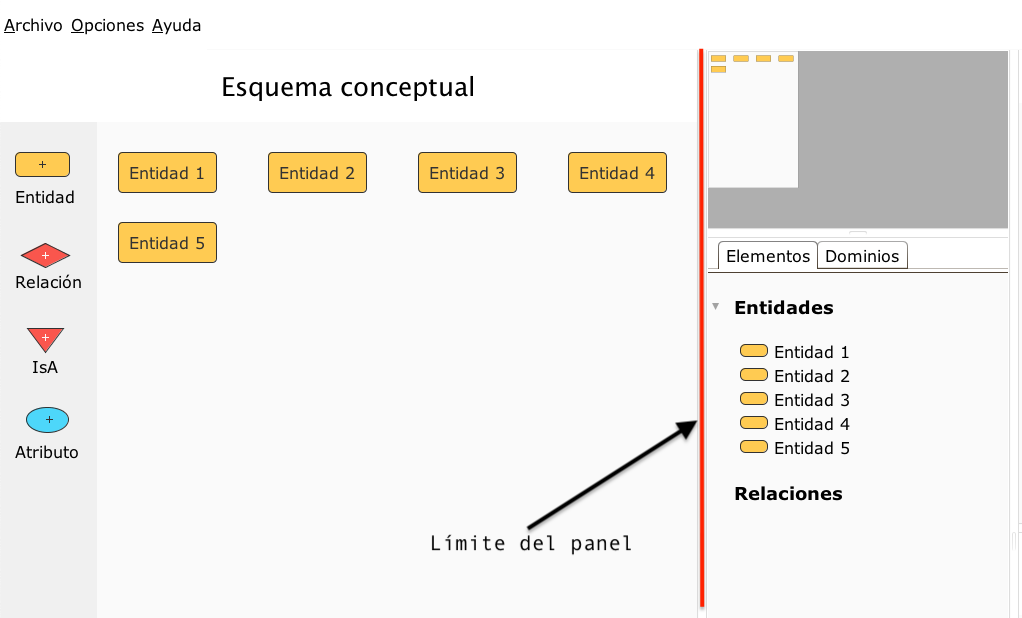
\includegraphics[width=0.8\textwidth]{img/limitepanel.png}
            \caption{Colocación de nuevos elementos}
        \end{figure}
        \item Los \textbf{atributos} siguen un comportamiento distinto
    \end{itemize}
\end{itemize}

\begin{comment}
- Disposicion de paneles
    - Panel de añadir elemento
    - Paneles de texto (HTML)
    - reporte de errores colorines
    - Cambios en el menú
    
- Perspectivas
- Diagrama
    - Colores
    - Formas redondeadas
    - Flechas

\end{comment}

%%%%%%%%%%%%%%%%
\section{Cambios a nivel de funcionalidad}
Los cambios a nivel de funcionalidad se han centrado principalmente en las traducciones desde el esquema conceptual a los esquemas lógico y físico. Se han corregido algunos errores arrastrados desde la versión anterior, y se han implementado nuevas traducciones, mejorando sobre todo el esquema lógico.

- Errores arrastrados
- guardar el estado de lenguaje, tema,
- Validacion automatica del diseño
- Exportación de los paneles por separado
- Nuevas cosas
- nullables

%%%%%%%%%%%%%%%%
\section{Cambios a nivel de codigo}
- Estructura de paneles
- Implementacion con git